%%%%%%%%%%%%%%%%%%%%%%%%%%%%%%%%%%%%%%%%%%%%%%%%%%%%%%%%%%%%
%%  This Beamer template was created by Cameron Bracken.
%%  Anyone can freely use or modify it for any purpose
%%  without attribution.
%%
%%  Last Modified: January 9, 2009
%%

\documentclass[xcolor=x11names,compress]{beamer}

%% General document %%%%%%%%%%%%%%%%%%%%%%%%%%%%%%%%%%
\usepackage{graphicx}
\usepackage{tikz}
\usetikzlibrary{arrows}
\usetikzlibrary{decorations.pathmorphing} % wiggly line
\usetikzlibrary{positioning} % relative positioning
\usetikzlibrary{fit} % box fitting
%%%%%%%%%%%%%%%%%%%%%%%%%%%%%%%%%%%%%%%%%%%%%%%%%%%%%%


%% Beamer Layout %%%%%%%%%%%%%%%%%%%%%%%%%%%%%%%%%%
\useoutertheme[subsection=false,shadow]{miniframes}
\useinnertheme{default}
\usefonttheme{serif}
\usepackage{palatino}

\setbeamerfont{title like}{shape=\scshape}
\setbeamerfont{frametitle}{shape=\scshape}

\setbeamercolor*{lower separation line head}{bg=DeepSkyBlue4} 
\setbeamercolor*{normal text}{fg=black,bg=white} 
\setbeamercolor*{alerted text}{fg=red} 
\setbeamercolor*{example text}{fg=black} 
\setbeamercolor*{structure}{fg=black} 
 
\setbeamercolor*{palette tertiary}{fg=black,bg=black!10} 
\setbeamercolor*{palette quaternary}{fg=black,bg=black!10} 

\renewcommand{\(}{\begin{columns}}
\renewcommand{\)}{\end{columns}}
\newcommand{\<}[1]{\begin{column}{#1}}
\renewcommand{\>}{\end{column}}
%%%%%%%%%%%%%%%%%%%%%%%%%%%%%%%%%%%%%%%%%%%%%%%%%%




\begin{document}


%%%%%%%%%%%%%%%%%%%%%%%%%%%%%%%%%%%%%%%%%%%%%%%%%%%%%%
%%%%%%%%%%%%%%%%%%%%%%%%%%%%%%%%%%%%%%%%%%%%%%%%%%%%%%
\begin{frame}
\title{A Program Logic for Verification of Security Properties in Secure
  ECMAScript}
\author{
  Thomas Wood \\[10pt]
  {\scriptsize
    Supervised by:\\[0pt]
    Dr. Gareth Smith \and Prof. Philippa Gardner
  } 
}
\titlepage
\end{frame}

%%%%%%%%%%%%%%%%%%%%%%%%%%%%%%%%%%%%%%%%%%%%%%%%%%%%%%
%%%%%%%%%%%%%%%%%%%%%%%%%%%%%%%%%%%%%%%%%%%%%%%%%%%%%%
\section{\scshape Background}
\begin{frame}{Secure ECMAScript}
  \begin{itemize}
    \item ECMAScript = JavaScript
    \item Secure ECMAScript (SES) -- language variant supporting \emph{Object
      capability} programming
    \item Key introduction: \emph{restricted evaluation}
  \end{itemize}
\end{frame}

\begin{frame}{Restricted Evaluation Example}
  \texttt{reval(\emph{code}, \emph{imports});}

  \texttt{reval(\emph{code}, \{a:a, b:b\});}
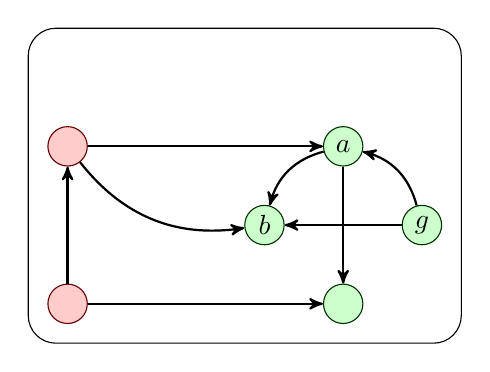
\begin{tikzpicture}[
    object/.style={circle, minimum size=5mm, inner sep=0},
    trusted/.style={object, draw=green!20!black, fill=green!20!white},
    untrusted/.style={object, draw=red!40!black, fill=red!20},
    membranec/.style={draw=blue, fill=blue!20},
    membrane/.style={object, membranec, minimum size=2mm},
    arrow/.style={thick, >=stealth'},
    pre/.style={arrow, <-},
    post/.style={arrow, ->}
  ]
  \draw[clip,rounded corners=10, use as bounding box] (0,0.5) rectangle (5.5,4.5);
  \node[trusted] (a) at (4,3) {$a$};
  \node[trusted] (b) at (3,2) {$b$}
    edge [pre,bend left] (a);
  \node[trusted] (g) at (5,2) {$g$}
    edge [post,bend right] (a)
    edge [post] (b);
  \node[trusted] (c) at (4,1) {}
    edge [pre] (a);

  \node[untrusted] (ua) at (0.5,3) {}
    edge [post] (a)
    edge [post,bend right] (b);
  \node[untrusted] (ub) at (0.5,1) {}
    edge [post] (ua)
    edge [post] (c);
\end{tikzpicture}
\end{frame}

\begin{frame}{Separation Logic}
\end{frame}

\begin{frame}{}
\end{frame}

\section{\scshape Project}
\begin{frame}{Modifying Separation Logic}
\end{frame}

\begin{frame}{New Inference Rules}
\end{frame}

\begin{frame}{Membrane Proof}
\end{frame}

\end{document}

